\documentclass{article}
\usepackage{graphicx} % Required for inserting images
\usepackage[utf8]{inputenc}
\usepackage{amsmath,amsfonts,amssymb,amsthm}
\usepackage{enumerate,bbm}
\usepackage{tikz,graphicx,color,mathrsfs,color,hyperref,boldline}
\usepackage{caption,float}
\usepackage[a4paper,margin=1in,footskip=0.25in]{geometry}

\usepackage{listings}
\usepackage{xcolor}

\usepackage{tabularx,capt-of}

\usepackage{blindtext}
%Image-related packages
\usepackage{graphicx}
\usepackage{subcaption}
\usepackage[export]{adjustbox}
\usepackage{lipsum}

%hyperref setup
\hypersetup{
    colorlinks=true,
    linkcolor=blue,
    filecolor=magenta,      
    urlcolor=cyan,
    pdftitle={Overleaf Example},
    pdfpagemode=FullScreen,
    }

%New colors defined below
\definecolor{codegreen}{rgb}{0,0.6,0}
\definecolor{codegray}{rgb}{0.5,0.5,0.5}
\definecolor{codepurple}{rgb}{0.58,0,0.82}
\definecolor{backcolour}{rgb}{0.95,0.95,0.92}

%Code listing style named "mystyle"
\lstdefinestyle{mystyle}{
  backgroundcolor=\color{backcolour}, commentstyle=\color{codegreen},
  keywordstyle=\color{magenta},
  numberstyle=\tiny\color{codegray},
  stringstyle=\color{codepurple},
  basicstyle=\ttfamily\footnotesize,
  breakatwhitespace=false,         
  breaklines=true,                 
  captionpos=b,                    
  keepspaces=true,                 
  numbers=left,                    
  numbersep=5pt,                  
  showspaces=false,                
  showstringspaces=false,
  showtabs=false,                  
  tabsize=2
}

%"mystyle" code listing set
\lstset{style=mystyle}

\theoremstyle{definition}
\newtheorem{defn}{Definition}[section]
\newtheorem{example}[defn]{Example}
\theoremstyle{remark}
\newtheorem{rem}{Remark}
\newtheorem{remS}[section]{defn}
\newtheorem{lem}[defn]{Lemma}
\theoremstyle{plain}
\newtheorem{thm}[defn]{Theorem}
\newtheorem{prop}[defn]{Proposition}
\newtheorem{fact}[defn]{Fact}
\newtheorem{crly}[defn]{Corollary}
\newtheorem{conj}[defn]{Conjecture}

%\newtheorem*{programming*}{Programming Task}

%\newtheorem{innercustomgeneric}{\customgenericname}
%\providecommand{\customgenericname}{}
%\newcommand{\newcustomtheorem}[2]{%
%  \newenvironment{#1}[1]
%  {%
%   \renewcommand\customgenericname{#2}%
%   \renewcommand\theinnercustomgeneric{##1}%
%   \innercustomgeneric
%  }
%  {\endinnercustomgeneric}
%}

%\newcustomtheorem{question}{Question}
%\newcustomtheorem{programming}{Programming Task}

\newcommand{\NN}{\mathbb{N}}
\newcommand{\ZZ}{\mathbb{Z}}
\newcommand{\QQ}{\mathbb{Q}}
\newcommand{\RR}{\mathbb{R}}
\newcommand{\CC}{\mathbb{C}}
\newcommand{\PP}{\mathbb{P}}
\newcommand{\FF}{\mathbb{F}}

\newcommand{\calD}{\mathcal{D}}
\newcommand{\id}{\operatorname{id}}

\newcommand{\sol}{\textit{Solution: }}
\newcommand{\Res}{\operatorname{Res}}

\title{Linear Analysis}
\author{Kevin}
\date{October 2024}

\begin{document}
\maketitle

\section{Normed spaces \& linear operators}
\begin{defn}
    Let $X$ be a vector space over $\RR$ or $\CC$ (usually over $\RR$). A \textbf{norm} on $X$ is a function $\Vert\bullet\Vert:X\to\RR_{\ge0}$ s.t. 
    \begin{enumerate}
        \item $\Vert x\Vert=0$ iff $x=0$;
        \item $\Vert\lambda x\Vert=|\lambda|\Vert x\Vert$ for all $x\in X$, $\lambda$ scalar;
        \item $\Vert x+y\Vert\le\Vert x\Vert+\Vert y\Vert$ for all $x,y\in X$ (Triangle inequality)
    \end{enumerate}
    A \textbf{normed space} is a pair $(X,\Vert\bullet\Vert)$, where $X$ is a vector space and $\Vert\bullet\Vert$ is a norm.
\end{defn}
\begin{example}
\begin{enumerate}
    \item $l_p^n$, $X=\RR^n$, $\Vert x\Vert=\Vert x\Vert_p=\left(\sum_i|x_i|^p\right)^{1/p}$. (Triangle inequality follows from Minkowski's inequality)
    \item $l_\infty^n$, $X=\RR^n$, $\Vert x\Vert=\Vert x\Vert_\infty=\max_i|x_i|$.
\end{enumerate}
\end{example}
\begin{rem}
    Often useful to consider the unit ball $B=B(X)$. $B$ completely determines the norm by $\Vert x\Vert=\inf\{t>0:x\in tB\}$. $B$ is always convex by triangle inequality. In fact, can check that if $B\subseteq\RR^n$ is a closed, bounded, convex, symmetric ($x\in B\implies -x\in B$), and is a nbd of $0$, then $B$ defines a norm via the formula above, and $B$ is the unit ball of that norm.
\end{rem}
Let $S$ be the set of scalar sequences made into a vector space under pointwise operations.
\begin{example}
    \begin{enumerate}
        \item $l_p=\{x\in S\colon \sum_i|x_i|^p<\infty\}$ with norm $\Vert x\Vert=\Vert x\Vert_p=\left(\sum_i|x_i|^p\right)^{1/p}$.
        \item $l_\infty=\{x\in S:\sup_n|x_n|<\infty\},\Vert x\Vert_\infty=\sup_n|x_n|$.
        \item $C_0=\{x\in S:x_n\to 0\}$ with norm $\Vert\bullet\Vert_\infty$.
    \end{enumerate}
\end{example}
\begin{defn}
    A Banach space is a complete normed space.
\end{defn}

\subsection{The H\"older \& Minkowski Inequality}
\begin{lem}
    For $1\le p<\infty$, $x\mapsto x^p$ is convex.
\end{lem}
\begin{thm}[Minkowski's inequality]
Let $1\le p<\infty$, $x,y\in l_p$, then $x+y\in l_p$ and $\Vert x+y\Vert_p\le\Vert x\Vert_p+\Vert y\Vert_p$.
\end{thm}
\begin{proof}
First assume $\Vert x\Vert_p,\Vert y\Vert_p\le 1$. For each $n$, we have 
\[|\lambda x_n+(1-\lambda) y_n|^p\le\lambda|x_n|^p+(1-\lambda)|y_n|^p\]
by the preceding lemma. So we have the same inequality of partial sums. Taking limit, we see that $\lambda x+(1-\lambda)y\in l_p$ and $\Vert \lambda x+(1-\lambda)y\Vert_p\le\lambda\Vert x\Vert_p+(1-\lambda)\Vert y\Vert_p$. For general $x,y\in l_p$, wlog assume $x,y\neq 0$ as otherwise the inequality is trivial. Apply the aove to the normalized vectors, we get
\[\Bigg\Vert\dfrac{\Vert x\Vert_p}{\Vert x\Vert_p+\Vert y\Vert_p}\dfrac{x}{\Vert x\Vert_p}+\dfrac{\Vert y\Vert_p}{\Vert x\Vert_p+\Vert y\Vert_p}\dfrac{y}{\Vert y\Vert_p}\Bigg\Vert_p\le 1\], which implies the claimed inequality after some manipulation.
\end{proof}
\begin{defn}
    $1\le p<\infty$, the conjugate index to $p$ is the $q$ s.t. $1<q<\infty$ with $1/p+1/q=1$.
\end{defn}
\begin{lem}
    If $p,q$ are conjugate, and $a,b\ge 0$, then $ab\le \frac{a^p}{p}+\frac{b^q}{q}$.
\end{lem}
\begin{proof}
    Can either do Legendre transform or substitute $x=a^p$, $y=b^p$ and use concavity of log.
\end{proof}
\begin{thm}[H\"older's inequality] If $p,q$ are conjugate, $x\in l_p$, $y\in l_q$, then $(x_ny_n)\in l_1$ with $\Vert (x_ny_n)\Vert_1\le\Vert x\Vert_p\Vert y\Vert_q$.
\end{thm}
\begin{proof}
    WLOG, assume $\Vert x\Vert_p=\Vert y\Vert_q=1$. For all $n$, $|x_ny_n|\le \frac{|x_n|^p}{p}+\frac{|y_n|^q}{q}$, so $(x_ny_n)\in l_1$ with $\Vert x_ny_n\Vert\le\frac{\Vert x\Vert_p^p}{p}+\frac{\Vert y\Vert_q^q}{q}=1/p+1/q=1$.
\end{proof}
\begin{example}
    \begin{itemize}
        \item $C([0,1])$ with the sup norm $\Vert f\Vert_\infty$ is complete (uniform convergence). More generally, $C(K)$ is with sup norm is complete if $K$ is compact Hausdorff.
        \item $C([0,1])$ with the $1$-norm $\Vert f\Vert_1=\int_0^1 f$ is incomplete. Still incomplete with $p$-norm $(\int_0^1 |f|^p)^{1/p}$.
        \item $C^1([0,1])$ of ctsly diff function with the sup norm $\Vert\bullet\Vert_\infty$ is incomplete. However with a new norm $\Vert f\Vert'=\Vert f\Vert_\infty+\Vert f'\Vert_\infty$, the space is complete (exercise)

    \end{itemize} The following result suggests that for a norm to be complete, one often needs to take into account the structure of the space.

    $\Delta=D^1\subseteq\CC$ the closed unit disk. $A(\Delta)$ be the space of functions which are cts on $\Delta$ and analytic on $\Delta^\circ$, then $A(\Delta)$ equipped with $\Vert f\Vert_\infty$ is complete (c.f. complex analysis, Montel's theorem, the uniform limit of holomorphic functions is holo'c).
\end{example}
\begin{rem}
    In $l_p$, ($1\le p\le\infty$). Write $e_n=(0,...,0,1,0,...)$ for the vector which is $1$ at the $n$th place. The linear span of $\{e_n\}$ is $F=\{x\in l_p:\exists N\ge 0,\forall n\in N,x_n=0\}\subsetneq l_p$. However, we get close for $1\le p<\infty$ since the closed linear span (the closure) of $e_n$ is $l_p$. To see this note that $\forall x\in l_p$, $\sum_{n=1}^k x_ne_n\to x$ as $k\to\infty$.

    The property above is false for $l_\infty$, e.g., take $(1,1,...)$. In fact the closed linear span in this case is $C_0$.

    Also note that Subspaces need not be closed, e.g. $F\subseteq l_1$ (even if $F$ is dense).
\end{rem}
\begin{defn}
    A topological space $X$ is separable if it has a countable dense subset.
\end{defn}
\begin{example}
    $l_p$ ($1\le p<\infty$) is separable (take finite rational sequences). $l_\infty$ is not separable (exercise).
\end{example}

\subsection{Linear Operators}
\begin{defn}
    $X,Y$ normed, a linear map $T:X\to Y$ is an operator if it's cts.
\end{defn}
\begin{prop}
    $X,Y$ normed, $T:X\to Y$ linear, then TFAE
    \begin{enumerate}
        \item $T$ cts
        \item $T$ cts at $0$
        \item $\exists k$ s.t. $\Vert T\Vert\le k\Vert x\Vert$ for all $x\in X$. ($T$ is bounded)
    \end{enumerate}
\end{prop}
\begin{proof}
    1 implies 2 is trivial. If 2 is true, then let $B(Y)$ be the unit ball in $Y$, which is a nbd of $0$, so by continuity at $0$, there exists $\delta>0$ s.t. $\Vert x\Vert<\delta\implies \Vert Tx\Vert\le 1$. Rearranging, get $\Vert Tx\Vert\le \Vert x\Vert/\delta$ for all $x\in B(Y)$, but then linearity allows us to say the same thing for all $x\in X$. To prove 3 implies 1, we simply note that Lipschitz condition implies continuity.
\end{proof}
\begin{defn}
    For bounded $T:X\to Y$, the operator norm of $T$ is $\Vert T\Vert=\sup\{\Vert Tx\Vert:\Vert x\Vert\le 1\}$.
\end{defn}
Then for all $x$, $\Vert Tx\Vert\le \Vert T\Vert\Vert x\Vert$.

We write $L(X,Y)$ for the set of cts linear maps $X\to Y$. In some sources, the notation $B(X,Y)$ is used.
\begin{rem}
    One can check that the operator norm is indeed a norm on $L(X,Y)$.
\end{rem}
\begin{prop}
    If $S:X\to Y$, $T:Y\to Z$ are operators, then $T\circ S$ is an operator and $\Vert TS\Vert\le \Vert T\Vert\Vert S\Vert$.
\end{prop}
\begin{proof}
    Direct computation.
\end{proof}
\begin{example}
    \begin{enumerate}
        \item $T:l_p^n\to l_p^n$ defined by projecting onto the first two coords. $\Vert T\Vert=1$.
        \item Right shift. This is an injective isometry, but not surjective.
        \item Left shift. This is surjective but not injective.
        \item $p,q$ conj. For $x\in l_p, y\in l_q$, write $x.y$ for $\sum x_ny_n$ which conv. abs. by H\"older. Can then define $\phi_y:l_p\to \RR$ by $x\mapsto x.y$. Have $\phi_y\in L(l_p,\RR)$ and $\Vert\phi_y\Vert\le \Vert y\Vert_q$.
        \item Take $(F,\Vert\bullet\Vert_1)$ and deifne $T:F\to \RR$, $x\mapsto \sum nx_n$. $T$ is linear but not cts.
        \item $T:l_1\to l_2$, $x\mapsto x$. Then $\Vert T\Vert=1$ as $\sum |x_n|\le 1\implies \forall n, |x_n|\le 1\implies\sum|x_n|^2\le 1\implies \Vert T\Vert\le 1$. $T$ is not surjective but the image contains $F$, so $\operatorname{im}(T)$ is dense. It is not closed so incomplete.
    \end{enumerate}
\end{example}
\begin{defn}
    $X,Y$ normed.
    \begin{itemize}
        \item The dual $X^\ast=L(X,\RR)$ with operator norm
        \item $X\to Y$ is an isomorphism if it's a linear homeo, i.e., $\exists c,d>0$ s.t. $c\Vert x\Vert\le\Vert Tx\Vert$ and $\Vert Tx\Vert\le d\Vert x\Vert$.
        \item  $X\to Y$ is an isometric isomorphism if it's an isometry.
        \item For isomorphic $X,Y$, the Banach-Mazur distance from $X$ to $Y$ is $d(X,Y)=\inf_{T \text{ iso}}\Vert T\Vert\Vert T^{-1}\Vert$.
        \item Two norms are equivalent if they induce the same topology, i.e., the identity is a homeo, i.e., two norms are Lipschitz equivalent. In particular, if two norms are equiv, and one of them is complete, then both are complete.
    \end{itemize}
\end{defn}
Note that for equivalent norms, $c\Vert x\Vert_1\le \Vert x\Vert_2\le d\Vert x\Vert_1$, i.e., $d^{-1}B_1\subset B_2\subset c^{-1}B$.
\begin{rem}
    \begin{itemize}
        \item On $C[0,1]$, $\Vert\bullet\Vert_\infty$ is complete, $\Vert\bullet\Vert_1$ is incomplete, so they are not equiv. The map $\operatorname{id}:(C[0,1],\Vert\bullet\Vert_\infty)\to(C[0,1],\Vert\bullet\Vert_1)$ is a cts linear bijection whose inverse is not cts.
        \item On $F$, $\Vert\bullet\Vert_1$ and $\Vert\bullet\Vert_2$ are not equiv. Take, $x=e_1+...+e_n$, then $\Vert x\Vert_1=n$, $\Vert x\Vert_2=\sqrt{n}$.
        \item $(T_n)$ a sequence in $L(X,Y)$ and $T_n\to T$ in operator norm, then $T_n\to T$ pointwise.
        The converse is false: $T_n:l_1\to \RR, x\mapsto x_n$. Then $\Vert T_n\Vert=1$ for all $n$, but we do have pointwise convergence.
    \end{itemize}
\end{rem}
\begin{thm}
    $X,Y$ normed, $Y$ complet. Then $L(X,Y)$ is complete with respect to the operator norm.
\end{thm}
\begin{proof}
    Given a Cauchy sequence $(T_n)$ in $L(X,Y)$, Pointwise, have
    $\Vert T_nx-T_my\Vert\le \Vert T_n-T_m\Vert\Vert x\Vert$, so pointwise Cauchy. Since $Y$ is complete, the pointwise limit exists. Can check that the pointwise limit $T$ is a linear map. It suffices to prove boundedness. Given $\epsilon>0$, there exists $N$ s.t. $\Vert T_m- T_n\Vert\le \epsilon$ for all $m\ge n\ge N$. Let $m\to \infty$, we get $\Vert Tx-T_nx\Vert\le\epsilon\Vert x\Vert$ for all $x$ and $n\in N$. So for all $x$, have
    \[\Vert Tx\Vert\le (\epsilon+\Vert T_m\Vert)\Vert x\Vert\]
    Note that $\Vert T_m\Vert$ is bounded as the sequence is Cauchy, so we have a uniform bound, so $T\in L(X,Y)$. Now, the preceding argument essentially says that $\Vert T-T_n\Vert\le\epsilon$ for all $n\ge N$.
\end{proof}
\begin{crly}
    If $X$ is a complete norm space, then $X^\ast$ is complete.
\end{crly}

We want to investigate the dual of $l_p$. Let $1<p,q<\infty$ be conjugate. For each $y\in l_q$, we defined $\phi_y\in l_p^\ast$. We know that $\Vert\phi_y\Vert\le\Vert y\Vert_q$. We construct $x_n=\operatorname{sgn}(y_n)|y_n|^{q/p}$, then $(x_n)\in l_p$ with $\Vert x\Vert_p=\Vert y\Vert_q^{q/p}$. $\phi_y(x)=\sum |y_n|^{q/p+1}=\sum |y_n|^q=\Vert y\Vert_q$. We see that $\Vert \phi_y\Vert=\Vert y\Vert_q$.
\begin{thm}
    Let $1<p,q<\infty$ be conjugate. Then $\theta:l_q\to l_p^\ast, y\mapsto \phi_y$ is an isometric isomorphism.
\end{thm}
\begin{proof}
    This map is obviously linear. It's norm preserving so obviously continuous and injective. To show surjectivity, consider $T\in l_q^\ast$ and define the following sequences (\textbf{important trick!}) $y_n=Te_n$.
    \[x_n=\begin{cases}
    \operatorname{sgn}(y_n)|y_n|^{q/p} & n\le N\\
    0 & \text{o/w}
    \end{cases}\]
    Then $x\in l_p$ and $Tx=\sum_1^N|y_n|^{q/p+1}=\sum_1^N|y_n|^q$, so $$\sum_1^N|y_n|^q\le\Vert T\Vert x\Vert_p=\Vert T\Vert\left(\sum_1^N|y_n|^q\right)^{1/p}$$
    so
    \[\Vert T\Vert\ge \left(\sum_1^N|y_n|^q\right)^{1/q}\]
    Let $N\to\infty$, we see that $y\in l_q$. By linearity and continuity, $T=\phi_y$ on $\overline{F}=l_q$.
\end{proof}
\begin{rem}
    \begin{enumerate}
        \item Same argument shows that $l_1^\ast=l_\infty$ and $C_0^\ast=l_1$ using the density of $\langle e_n:n\in \NN\rangle$.
        However, it wouldn't show $l_\infty^\ast=l_1$. In fact, there exists $T\in l_\infty^\ast$ not of the form $\phi_y$. The proof of this fact is beyond the scope of this course.
        \item Each $l_p$ ($1\le p\le \infty$) is complete and each is a dual space
        \item Cannot have $X^\ast=\{0\}$ by Hahn-Banach theorem (Any cts functional on a subspace extend to a continuous functional on the whole space).
    \end{enumerate}
\end{rem}
\subsection{Finite Dimensional Spaces}
\begin{thm}
    Any two norms on a finite dimensional vector space are equivalent.
\end{thm}
\begin{proof}
    Will show that any norm on $\RR^2$ is equiv to $\Vert -\Vert_\infty$. For $x\in\RR^n$, $\Vert x\Vert\le\sum\Vert x_ie_n\Vert=\sum|x_i|\Vert e_i\Vert\le n(\max_i\Vert e_i\Vert)\Vert x\Vert_\infty$.

    Conversely, consider $f:S\to \RR$, where $S=\{x\in\RR^n:\Vert x\Vert_\infty=1\}$, then $f$ is continuous on compact set so there eixsts $\delta>0$ s.t. $\Vert x\Vert_\infty=1\implies \Vert x\Vert\ge \delta$, so if $0\neq x\in\RR^n$, then $x=\Vert x\Vert_\infty\hat{x}$ and $\Vert x\Vert\ge \delta\Vert x\Vert_\infty$.
\end{proof}
\begin{crly}
    $X,Y$ normed and $\dim X<\infty$, then every lienar map $T:X\to Y$ is cts.
\end{crly}
\begin{proof}
    Define norm on $X$ yb $\Vert x\Vert'=\Vert x\Vert+\Vert Tx\Vert$, so there exists $c$ s.t. $\Vert x\Vert'\le c\Vert x\Vert$ by equivalence of norm, so $\Vert Tx\Vert\le c\Vert x\Vert$ by unwinding a bit.
\end{proof}
\begin{crly}
    $X,Y$ finite dim normed spaces of with $\dim X=\dim Y$. Then $X,Y$ are isomorphic.
\end{crly}
\begin{crly}
    \begin{enumerate}
        \item $Y$ normed finite dim vec space, then $Y$ complete;
        \item $X$ normed, then if $Y\subset X$ is a finite dim subspace then $Y$ is closed.
    \end{enumerate}
\end{crly}
\begin{crly}
    If $X$ is a finite dim normed vec space then $B_x$ is compact (being closed and bounded in 2-norm).
\end{crly}
Note that the unit ball in $l_p$ is not compact since $\Vert e_i-e_j\Vert\ge 1$ for all $i,j$.

Define $d(x,Y)=\inf\{d(x,y):y\in Y\}$ as the distance from $x$ to a closed subspace $Y$. Note that $d(x,Y)=0$ iff $x\in Y$ (closed).
\begin{prop}[Riesz's lemma]
    If $X$ is normed and $Y$ a proper closed subspace of $X$, then for all $\epsilon>0$, there exists $x\in X$ with $\Vert x\Vert=1$ s.t. $d(x,Y)\ge 1-\epsilon$. Moreover, if $\dim X<\infty$, then $\exists x\in X$ s.t. $\Vert x\Vert =1$ with $d(x,Y)=1$.
\end{prop}
\begin{proof}
    Let $\epsilon>0$ be given.
    Choose $x\in X$ s.t. $x\in Y$ and $\Vert x\Vert=1$. Pick $y\in Y$ with $\Vert x-y\Vert\le (1+\epsilon)d(x,Y)$. Define $z=\frac{x-y}{\Vert x-y\Vert}$. Can check that for any $y'\in Y$, we have
    \[z-y'=\dfrac{x-y-\Vert x-y\Vert y'}{\Vert x-y\Vert}\ge \dfrac{d(x,Y)}{\Vert x-y\Vert}\ge \dfrac{1}{1+\epsilon}\]
    For the second part, note that $d(x,Y)$ is a cts function $B_X\to\RR$. The domain is compact if $X$ is finite dimensional, so attains its lower bound.
\end{proof}
\begin{thm}
    $X$ infinite dim normed space. Then there eixsts a seq. $(x_n)$ in $X$ with $\Vert x\Vert=1$ for all $n$ and $\Vert x_n-x_m\Vert\ge 1$ for all $m\neq n$. In particular, $B_X$ is not compact.
\end{thm}
\begin{proof}
    Choose $x_1\in X$ with unit norm. Inductively set $Y=\langle x_1,...,x_n\rangle$ and $X'=\langle x_1,...,x_n,x\rangle$ for any $x\not\in Y$. By Riesz's lemma, there exists $x_{n+1}\in X'$ s.t. $\Vert x_{n+1}\Vert=1$ and $d(x_{n+1},Y)=1$.
\end{proof}

\subsection{Compact Operators}
\begin{defn}
    $X,Y$ normed. A linear operator $T:X\to Y$ is compact if $\overline{T(B_X)}$ is compact.
\end{defn}


\begin{example}
    For instance, if $T$ has finite rank, then $\overline{T(B_X)}$ is closed and bounded in finite dimensional space hence compact.

    If $X$ is infinite dimensional, then $\operatorname{id}_X$ is not compact due to the preceding theorem.
\end{example}
\begin{rem}
    \begin{enumerate}
        \item Compact implies cts.
        \item Note that if $Y$ is complete, then $T$ is compact if and only if $T(B_X)$ is totally bounded. 
        \item $T:X\to Y$ is compact iff for any $(x_n)$ in $B_X$, there exists a subsequence $(x_{n_i})$ with $T(x_{n_i})$ convergent.
    \end{enumerate}
\end{rem}

\begin{prop}
    $X,Y$ normed. $Y$ complete. Then $\{\text{compact operators}\}$ is a closed subspace of $L(X,Y)$.
\end{prop}
\begin{proof}
    Take a sequence $(x_n)$ in $B_X$. then can find a subsequence whose image under $S$ converges. Pass to some subsequence of this subsequence so that the image under $T$ also converges, so if $S,T$ are compact then so is $S+T$. This implies that the space of compact operators form a subspace.

    Consider a sequence $T_n\to T$ for $T_n$ compact. Given $\epsilon>0$, choose $n$ with $\Vert T_n-T\Vert<\epsilon$. Since $T_n(B_X)$ is totally bounded, we have $T_n(B_X)=\bigcup_{i=1}^mB(T_n(x_i),\epsilon)$ for some $x_i$. So, $T(B_X)\subseteq\bigcup_iB(T_n(x_i),2\epsilon)$ and $T(B_X)\subseteq\bigcup_i B(T(x_i,3\epsilon))$, which gives total boundedness. 
\end{proof}
In particular, the limit of finite rank operators is compact.
\begin{example}
    For fixed $1\le p\le\infty$, the projection onto the $n$th coord $p_n$ is a finite rank operator with $\Vert p_n\Vert=1$. $p=\sum_np_n/n^2$ converges as it's Cauchy, then $p$ is compact but not of finite rank.
\end{example}
\begin{prop}
    $X,Y,Z$ normed, $S\in L(X,Y)$, $T\in L(Y,Z)$, then
    \begin{enumerate}
        \item $S$ compact $\implies T\circ S$ compact
        \item $T$ compact $\implies T\circ S$ compact.
    \end{enumerate}
\end{prop}
\begin{proof}
    To prove the first claim, consider a sequence $(x_n)$ in $B_X$, then there is a subsequence with $S{x_{n_i}}$ convergent, so $TSx_{n_i}$ is convergent by continuity.

    To prove the second claim. Note that for any sequence $(x_n)$ in $B_X$, $Sx_n$ is bounded, so $TSx_{n_i}$ converges for some subsequence as $T$ is compact.
\end{proof}
We have seen the map $T:l_1\to l_2$ with dense image but not all of $l_2$. For instance $x(1/\sqrt{n},...,1/\sqrt{n},0,0,...)$ then $\Vert x\Vert_2=1$ $\Vert x\Vert_1=\sqrt{n}$.

\begin{thm}[Open mapping lemma]
    $X,Y$ normed. $X$ complete, then $T\in L(X,Y)$. Suppose $\overline{T(B_X)}\supset B_Y$, then
    \begin{enumerate}
        \item $\forall y\in Y,\exists x\in X$ s.t. $Tx=y$ and $\Vert x\Vert\le 2\Vert y\Vert$ (In particular, $T$ is surjective.)
        \item $Y$ complete.
    \end{enumerate}
\end{thm}
\begin{rem}
    \begin{enumerate}
        \item $\overline{T(B_X)}\supset B_Y$ implies that the image of $B_X$ is dense in $B_Y$, i.e., $\forall y\in B_Y,\forall\epsilon>0$, $\exists x\in B_X$ with $\Vert Tx-y\Vert<\epsilon$.
        \item The proof would also show that for all $y\in Y$, there eixsts $x$ with $\Vert x\Vert\le|1+\epsilon|\Vert y\Vert$ for any fixed $\epsilon$.
        \item We say that $T$ is open if the image of any open set is open, i.e., $T(B_X)$ is a nbd of $0$, i.e., $T(B_X)\supset\frac{1}{k}B_Y$ for some $k\in\NN$, i.e., $\forall y\in Y,\exists x\in X$ with $Tx=y$ and $\Vert x\Vert\le k\Vert y\Vert$. Therefore, open mapping lemma says that if $\operatorname{im}(B_X)$ is desne in $B_Y$, then $T$ is open.
    \end{enumerate}
\end{rem}
\begin{proof}
    \begin{enumerate}
        \item Given $y\in Y$ with unit norm. Seek $x\in X$ with $Tx=y$ and $\Vert x\Vert\le 2$. $T(B_X)$ is dense in $B_Y$, so $\exists x_1\in X$ s.t. $\Vert x_1\Vert\le1$ and $\Vert y-Tx_1\Vert\le 1/2$. Also, $T(\frac{1}{2}B_X)$ is dense in $1/2B_Y$, so $\exists x_2\in X$ with $\Vert x_2\Vert\le 1/2$ s.t. $\Vert y-T(x_1+x_2)\Vert\le 1/4$. Continue, obtain $x=\sum x_n$ which is Cauchy, hence convergent, and $\Vert y-Tx\Vert=0$, so $Tx=y$.
        \item Given $(y_n)$ Cauchy in $Y$. WLOG assume $\Vert y_n-y_{n-1}\Vert\le 2^{-n}$ (by passing to a subsequence if necessary). For each $n\ge 2$, choose $x_n\in X$ s.t. $\Vert x_n\Vert\le 2^{-n+1}$ with $Tx_n=y_n-y_{n+1}$. Also, choose $x_1\in X$ with $Tx_1=y_1$ (surjectivity). Thus $T(x_1+...+x_n)=y_n$. Put $x=\sum x_n$ which is Cauchy hence convergent. Then $Tx=\lim_n T(\sum_1^n x_i)=\lim y_n$, so $y_n$ converges. 
    \end{enumerate}
\end{proof}
\subsection{New Spaces From Old}
\begin{defn}[Direct sum]
    $X\oplus_p Y$ ($1\le p\le\infty$), where $\Vert(x,y)\Vert_p=(\Vert x\Vert^p+\Vert y\Vert^p)^{1/p}$ and $\Vert (x,y)\Vert_\infty=\sup(\Vert x\Vert,\Vert y\Vert)$.
\end{defn}
These norms are all equivalent, so we usually write $X\oplus Y$.
If $X,Y$ are Banach then so is $X\oplus Y$. $X,Y$ are always closed subspaces of $X\oplus Y$.
\begin{defn}[Quotient]
    $X$ normed, $N\le X$ a closed linear subspace. We can define the quotient space $X/N$. Define $\Vert z\Vert =\inf\{\Vert x\Vert:x\in X,\pi(x)=z\}$, where $\pi:X\to X/N$ is the canonical projection map (continuous in this norm). If $X$ is Banach, then so is $X/N$.
\end{defn}
\begin{proof}
    The only non-trivial property to check is positivity. If $\Vert z\Vert=0$ for some $z\in X/N$,
    then there exists $x_1,x_2,...\in X$  with $\pi(x_n)=z$ and $\Vert x_n\Vert\to 0$. Then let $\pi(x)=z$, we have $x_n\to 0$ and $x_n-x\in N$, so $x\in N$ as $N$ is closed, so $z=0$.

    Clear that the projection is cts as $\Vert\pi(x)\Vert\le \Vert x\Vert$ by definition.

    If $X$ is Banach, then $\forall z\in X/N$ with $\Vert z\Vert\le 1$, there exists $x\in X$ with $\Vert x\Vert <1$ with $\pi(x)=z$, so $\pi(B_X)$ is dense in $B_{X/N}$. Done by open mapping lemma.
\end{proof}

\begin{defn}[Completion]
    $X$ normed, there exists a completion of $X$ defined as
    \[\Tilde{X}=\{\text{Cauchy sequences in }X\}/{\sim}\]
    where $(x_n)\sim(y_n)$ iff $x_n-y_n\to 0$. This is naturally a vector space equipped with the norm $\Vert[(x_n)]\Vert_{\Tilde{X}}=\lim\Vert x_n\Vert$. Then $\Tilde{X}$ is complete and $X$ is a dense subspace of $\Tilde{X}$ given by embedding $x\mapsto(x,x,x,...)$.
\end{defn}
Warning: 1st iso fails, e.g., $l_1\to l_2, x\mapsto x$ is injective, but the image is not complete.

\section{Baire Category Theorem}
\begin{thm}[Baire Category Theorem]
    $X$ non-empty complete metric space and $O_1,O_2,...$ a sequence of dense open sets. Then $\bigcap_{n\ge 0}O_n\neq\varnothing$.
\end{thm}
\begin{proof}
    $O_1\neq\varnothing$, so $\exists \overline{B(x_1,\epsilon_1)}\subseteq O_1$ for some $x_1$ and $\epsilon<1$. $O_2$ is dense, so can find $\overline{B(x_2,\epsilon)}\subseteq B(x_1,\epsilon_1)\cap O_2$ for some $x_2$ and $\epsilon_2<1/2$. Continue, get a nested sequence of closed balls. We have $\epsilon_n\to 0$ and $\overline{B(x_n,\epsilon_n)}\subseteq O_n$. $(x_n)$ is Cauchy so converges by completeness, so $x_n\in x\in\bigcap_nO_n$.
\end{proof}
\begin{rem}
    Cannot omit ``dense'' (e.g., $(0,1),(2,3)$ in $\RR$) or ``open'' (e.g. $\QQ,\RR\setminus\QQ\subseteq\RR$), or ``complete'' (e.g. $O_n=\QQ\setminus\{q_n\}$, where $q_1,...$ is an enumeration of rationals in $\QQ$.)

    The exact same proof shows that $\bigcap_n O_n$ is dense in $X$.
\end{rem}
Note that $O$ open dense iff $O^c$ closed and has empty interior.
\begin{thm}[BCT']
    $X$ non-empty complete metric space. $F_1,F_2,...$ closed in $X$ with $\bigcup_n F_n=X$ Then some $X$ has non-empty interior.
\end{thm}
\begin{defn}
    $A\subset X$ (metric) is nowhere dense (ND) if it's not dense in any open ball, i.e., $A^\circ=\varnothing$.
\end{defn}
It is clear that $A$ ND iff $\overline{A}$ ND. If $A$ is closed, then $A$ ND iff $A$ contains no open ball.
\begin{thm}[BCT'']
    $X$ non-empty complete metric space. $A_1,...$ ND subsets of $X$, then $\bigcup_n A_n\neq X$.
\end{thm}
\begin{defn}
    $A\subset X$ (metric) is meager if $A=\bigcup_nA_n$, $A_n$ ND for all $n$. (Countable union of ND subsets)
\end{defn}
Then BCT'' implies that $X$ is not a meager subset of $X$.

Note that there exists uncountable ND subset of $[0,1)$, i.e., the Cantor set $\{\sum_na_n3^{-n}:a_n=0\text{ or }2\}$.

\subsection{Applications of BCT}
\begin{prop}[Osgood's Theorem]
    If $(f_n)$ is a sequence of cts functions on $[0,1]$ which is pointwise bounded, then there exists $a<b$ s.t. $f_n$ is unif. bounded on $(a,b)\subseteq[0,1]$.
\end{prop}
\begin{proof}
    Define $E_n=\{x\in[0,1]:\forall i, |f_i(x)|\le n\}$, then $\bigcup_nE_n=[0,1]$ and $E_n$ is closed for all $n$, so some $E_n$ has non-empty interior.
\end{proof}
\begin{thm}[Principle of uniform boundedness]
$X$ Banach, $Y$ normed. Let $T_1,T_2,...,\in L(X,Y)$. If $(T_n)$ is pointwise bounded. Then $T_n$ are uniformly bounded.    
\end{thm}
\begin{proof}
    Define $E_n\{x\in X:\forall i,\Vert T_i(x)\Vert\le n\}$ (closed, cover $X$), so there exists $B(x,\epsilon)\subseteq E_n$ for some $n,x,\epsilon$. So for any $y\in X$ s.t. $\Vert y\Vert<\epsilon$, $x,x+y\in B(x,\epsilon)$. So $\forall i$, $\Vert T_iy\Vert=\Vert T_i(x+y)-T_i(x)\Vert\le 2n$, so $\Vert T_i\Vert\le 2n/\epsilon$.
\end{proof}
\begin{thm}[Banach-Steinhaus Theorem]
    $X$ Banach, $Y$ normed, $T_1,T_2,...\in L(X,Y)$ s.t. $T_n\to T$ pointwise. Then $T\in L(X,Y)$ (linear and cts)
\end{thm}
\begin{proof}
    Linearity is trivial. Need to show continuity.
    $\forall x\in X$, $T_nx\to Tx$ so $T_n$ is pointwise bounded hence uniformly bounded by principle of uniform boundedness. So $\exists M$ s.t. $\Vert T_n\Vert\le M$ for all $n$, so $\Vert T_nx\Vert\le\Vert T_n\Vert \Vert x\Vert\le M\Vert x\Vert$. Let $n\to\infty$, we see that $\Vert Tx\Vert\le M\Vert x\Vert$.
\end{proof}
\begin{thm}[Open Mapping Theorem]
    $X,Y$ Banach, $T\in L(X,Y)$ surjective. Then $T$ is an open map [$\exists R$ s.t. $\forall y\in Y$ $\exists x\in X$ s.t. $Tx=y$ with $\Vert x\Vert \le R\Vert y\Vert$.]
\end{thm}
\begin{proof}
    $T$ is surjective, so $\bigcup_n\overline{T(nB_X)}=Y$ which each $\overline{T(nB_X)}$ closed. Baire $\implies$ that some $T(nB_X)$ contains a ball $B(y,\epsilon)$. WLOG, $n=1$, so $T(B_X)$ is dense in $B(y,\epsilon)$. Now for all $z\in Y$ with $\|z\|<\epsilon$, we have $y+z,y-z\in B(y,\epsilon)$, so there exists $x,x'\in B_X$ with $\| Tx-(y+z)\|<\delta$ and $\|Tx'-T(y-z)\|<\delta$, which implies that $\frac{x-x'}{2}\in B_X$ and $\| T((x-x')/2)-z\|<\delta/2+\delta/2=\delta$. So $T(B_X)$ is dense in $B(0,\epsilon)$. By open mapping lemma (applied to the operator $T/\epsilon$), there exists $x\in X$ with $Tx=\epsilon y$ with $\|x\|\le 2\|y\|$, i.e., $T(x/\epsilon)=y$ and $\|x/\epsilon\|\le \frac{2}{\epsilon}\|y\|$.
\end{proof}
\begin{crly}[Inversion Theorem]
    $X,Y$ Banach. $T\in L(X,Y)$ bijective, Then $T$ is an isomorphism
\end{crly}
\begin{proof}
    $T$ surjective, so $T$ is open by open mapping thm, so $\exists k$ s.t. $\forall y\in Y$, $\Vert T^{-1}y\Vert\le k\Vert y\Vert$, so $T^{-1}$ is cts.
\end{proof}
\begin{crly}[Comparability theorem]
    Let $\|\ \|_1$, $\|\ \|_2$ be complete norms on $V$. If $\exists c>0$ s.t. $\forall x,\ \|x\|_2\le c\|x\|_1$. Then these two norms are equivalent.
\end{crly}
\begin{proof}
    Note that $\id:(V,\|\ \|_1)\to(V,\|\ \|_2)$ is a continuous bijection. Done by inversion theorem.
\end{proof}
\begin{thm}[Closed graph theorem (CGT)]
    $X,Y$ Banach, $T\in L(X,Y)$. Then $T$ is cts iff $\operatorname{Graph}(T)$ is closed.
\end{thm}
\begin{rem}
    This has an important consequence. $T$ has closed graph $\Leftrightarrow$ If $(x_n,Tx_n)\to (x,y)$, then $y=Tx$. $\Leftrightarrow$ If $x_n\to x$ and $Tx_n\to y$, then $y=Tx$. $\Leftrightarrow$ If $x_n\to 0,\ Tx_n\to y$, then $y=0$.

    CGT $\implies$ to show $T$ cts, it suffices to show that if $x_n\to 0$ and $Tx_n\to y$ (can assume the existence of this limit) then $y=0$.
\end{rem}
\begin{proof}
    ``$\Rightarrow$'': Trivial.

    ``$\Leftarrow$'': Let $G(T)$ denote the graph of $T$. $G(T)$ is closed in $X\times Y$ (with $\|\ \|_1$ say) by assumption, so $G(T)$ is complete. Define $S:X\to G(T),\ x\mapsto (x,Tx)$ WTS that $S$ is bounded. Clearly $S$ is a bijection and $S^{-1}$ is cts ($\|x\|\le \|x\|+\|Tx\|$), so we are done by inversion theorem.
\end{proof}
\subsubsection{Existence of a cts nowhere differentiable function}
$f\in C[0,1]$ is diffrentiable at $x$ iff $\frac{f(x+t)-f(x)}{t}\to 0$ as $t\to 0$. In particular the difference quotient is bounded for all $t\neq 0$ small. Define $E_n=\{f\in C[0,1]:\exists x,\ \forall t,\ |(f(x+t)-f(x))/t|\le n\}$

\textbf{Claim: $E_n$ is closed}: Suppose $(f_i)\in E_n$ with $f_i\to f$ unif. For each $i$, there exists $x_i$ s.t. $|(f_i(x_i+t)-f_i(x_i))/t|\le n$ for all $t$. By passing to a convergent subsequence if necessary, we may assume $x_i\to x$ as $i\to\infty$ for some $x\in [0,1]$. Then have
\[\dfrac{f_i(x_i+t)-f_i(x_i)}{t}-\dfrac{f(x+t)-f(x)}{t}\]
for all $t$. Thus, $|(f(x+t)-f(x))/t|\le n$ for all $t$, so $f\in E_n$.

\textbf{Claim: $E_n$ is nowhere dense (ND).} Given $f\in E_n$ and $\epsilon>0$, we need $g\in B(f,3\epsilon)$ with $g\not\in E_n$. By uniform continuity of $f$, we can find $\delta>0$ s.t. $|x-y|<\delta\implies |f(x)-f(y)|<\epsilon$. Take the following function. to be $g$.
\begin{figure}[H]
    \centering
    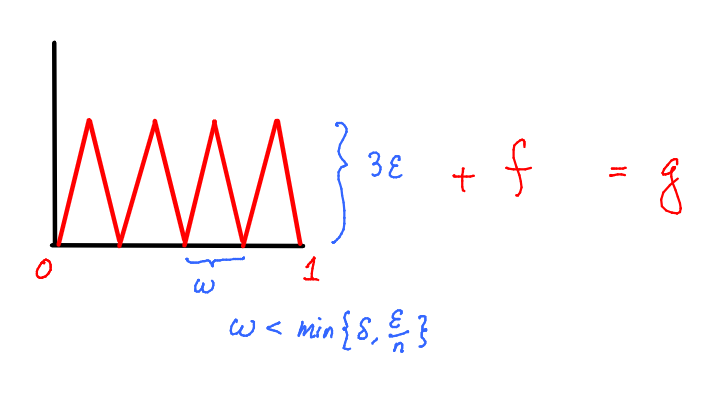
\includegraphics[width=0.5\linewidth]{Mich/pictures/LA-non-diff-func.PNG}
\end{figure}
Then we are done by Baire.

\section{Spaces of Continuous Functions}
\subsection{Existence of Continuous Functions}
\begin{defn}
    A Hausdorff space $X$ is normal if any two disjoint closed sets can be separated by two disjoint open sets.
\end{defn}
\begin{prop}
    Compact Hausdorff $\implies$ Normal.
\end{prop}
\begin{proof}
    Part IB Analysis and Topology ES3 Q8.
\end{proof}
\begin{thm}[Urysohn's lemma]
    Let $X$ be normal, $A,B\subseteq X$ be disjoint closed sets. Then $\exists$ a cts function $f:X\to[0,1]$ s.t. $f\equiv 0$ on $A$ and $f\equiv 1$ on $B$. 
\end{thm}
\begin{rem}
    \begin{itemize}
        \item Usually use normality in the following equivalent form. For $A\subseteq V$ where $A$ is closed and $V$ is open, there exists an open $U$ with $A\subseteq U$ and $\bar U\subseteq V$.
        \item If $X$ is Hausdorff and has the property in Urysohn lemma, then $X$ is normal. Take $f^{-1}(\{1/4\})$ and $f^{-1}(\{3/4\})$, so this characterizes normal spaces.
        \item This is trivial for metric spaces. Take $f(x)=\frac{d(x,A)}{d(x,A)+d(x,B)}$.
        \item If $K$ is compact Hausdorff (and infinite), then $C(K)$ is infinite dimensional. Pick an infinite sequence $(x_n)$ with distinct terms (possible as the set is infinite). For $n\ge 2$, pick $f_n\in C(K)$ with $f_n=0$ on $\{x_1,...,x_n\}$ and $f_n=1$ on $\{x_{n+1}\}$. It's easy to see that $\{f_n\}$ is an L.I. set.
     \end{itemize}
\end{rem}
\begin{proof}
    Let $A,B\subseteq X$ be disjoint closed sets. Let $V=B^c$. Find $O_{1/2}$ open s.t. $A\subseteq O_{1/2}$ and $\bar O_{1/2}\subseteq V$. Continue, find $O_{1/4}, O_{3/4}$ with $A\subseteq O_{1/4},\ \bar O_{1/4}\subseteq O_{1/2}$ and $\bar O_{1/2}\subseteq O_{3/4},\ \bar O(3/4)\subseteq V$. Continue, we get $O_q$ for all dyadic rational $q\in (0,1]$. The family $\{Q_q\}$ has the properties that
    \begin{itemize}
        \item $A\subseteq O_q\subseteq V$ for all $q$;
        \item $\bar O_q\subseteq O_r$ if $q<r$;
        \item Define $O_1=X$.
    \end{itemize}
    Define $f(x)=\inf\{q:x\in O_q\}$. To show continuity, it is enough to consider the preimages of $(-\infty,a)$ and $(-\infty,a)$. for $a\in(0,1)$.
    \begin{itemize}
        \item $f(x)<a\Leftrightarrow x\in O_q$ for some $q<a$, $\Leftrightarrow x\in\bigcup_{q<a}O_q$ which is open;
        \item $f(x)>a\Leftrightarrow x\not\in O_q$ for some $q>a$, i.e., $x\not\in\bar O_r$ for some $r>a$ $\Leftrightarrow x\in\bigcup_{r>a}\bar O_r^c$ open.
    \end{itemize}
\end{proof}
\begin{thm}[Tietze extension theorem]
    $X$ normal, $Y\subseteq X$ closed, $f:Y\to \RR$ bounded cts. Then $f$ extends to a cts function $g:X\to \RR$ with $\|g\|_\infty=\|f\|_\infty$.
\end{thm}
\begin{rem}
    \begin{itemize}
        \item The condition $\|g\|=\|f\|$ is trivial. If $g:X\to\RR$ extends to $f$ with $\|f\|=1$, then the map \[g'(x)=\begin{cases}
            g(x) & g(x)\in[-1,1]\\
            1 & g(x)>1\\
            -1 & g(x)<-1
        \end{cases}\]
        also extends $f$ ctsly.
        \item $Y$ being closed is necessary, e.g., $\sin(1/x)$ on $(0,1]\subseteq[0,1]$.
        \item Tietze extends the result of Urysohn lemma.
    \end{itemize}
\end{rem}
\begin{proof}
    WLOG, $\|f\|=1$. Let $A=\{x\in Y:f(x)<-1/3\}$, $B=\{x\in Y:f(x)>1/3\}$. By Urysohn, there exists a cts $g_1:X\to [-1/3,1/3]$ with $g_1=-1/3$ on $A$ and $g_1=1/3$ on $B$. Note that $|f(x)-g_1(x)|\le 2/3$ for all $x\in Y$, so $\|f-g_1\|_\infty\le2/3$. Repeat the process with $(f-g)$ in place of $f$ to obtain $g_2:X\to[-2/9,2/9]$ s.t. $\|f-g_1-g_2\|\le (2/3)^2$. We thus get a sequence of cts functiosn $g_1,g_2,...:X\to\RR$, s.t. $\|g_n\|\le\frac13(\frac23)^{n-1}$ and $\|f-\sum_{i=1}^ng_i\|_\infty\le(\frac23)^n\to0$ as $n\to\infty$. Let $g=\sum_ig_i$ which converges (being uniformly Cauchy). Have $\|g\|_\infty\le 1$ (can bound this by a geometric series), and $\|f-g|_Y\|=0$, so $f=g|_Y$.
\end{proof}\
\begin{proof}
    One can also proceed slightly differently by applying Riesz's lemma and open mapping lemma. The image of the restriction map is dense, and each function in the image of some function of the same sup norm. Open mapping lemma then implies that the restriction map is surjective.
\end{proof}

\subsection{Compactness in $C(K)$}
\begin{defn}
    For $K$ compact Hausdorff and $S\subseteq C(K)$, $S$ is equicontinuous at $x$ if 
    \[\forall\epsilon>0,\ \exists\text{ nbd } N\ni x\text{ s.t. }\forall f\in S,\ y\in N\implies |f(x)-f(y)<\epsilon\]
    We say that $S$ is equicontinuous if it is equicontinuous at $x$ for every $x\in K$.
\end{defn}
\begin{example}
    $\{\sin(n+x):n\in\NN\}$ is equicontinuous since $|x-x'|<\epsilon\implies |f(x)-f(x')|<\epsilon$ (MVT + all derivatives $\le 1$). But $\{\sin(nx):n\in\NN\}$ is not equicontinuous at $0$.
\end{example}
\begin{thm}[Arzela-Ascoli]
    Let $K$ be compact Hausdorff and $S\subseteq C(K)$. Then $S$ is compact if and only if $S$ is closed, bounded and equicontinuous.
\end{thm}
\begin{proof}
    `$\Rightarrow$': If $S$ is compact, then it is closed and totally bounded (hence bounded) by IB analysis and topology. Let $\epsilon>0$ be given. Let $x\in K$. Since $S$ is totally bounded, we can find $f_1,...,f_n\in S$ s.t. $S\subseteq \bigcup_{i=1}^nB(f_i,\epsilon)$. For each $i$, $f_i$ is continuous at $x$, so there exists open $U_i$ with $x\in U_i$ s.t. $\forall y\in U_i,\ |f_i(y)-f_i(x)|<\epsilon$. Let $U=\bigcap_{i=1}^n U_i$. Then $U$ is an open nbd of $x$ and $\forall y\in U$ and $\forall i$, $|f_i(y)-f_i(x)|<\epsilon$. But then for any $f\in S$, we have $\|f-f_i\|_\infty<\epsilon$ for some $i$. Therefore $$\forall y\in U,\ |f(y)-f(x)|\le |f(y)-f_i(y)|+|f_i(y)-f_i(x)|+|f_i(x)-f(x)|<3\epsilon$$

    `$\Leftarrow:$': Conversely $S$ is closed, so sufficient to prove total boundedness. Given $\epsilon>0$, we know that $S$ is equicontinuous, so $\forall x\in K$, there exists open $U_x\ni x$ s.t. $\forall f\in S$, $\forall y\in U_x$: $|f(y)-f(x)|<\epsilon$. Then $(U_x)_{x\in K}$ is an open cover of $K$. By compactness of $K$, we can reduce to a fintie subcover, say $K=U_{x_1}\cup...\cup U_{x_n}$. For $f\in S$ define $\hat f\in\RR^n$ by $\hat f=(f(x_1),...,f(x_n))$. $\hat f$ contains all the information of $f$ up to $\epsilon$. Let $\hat S=\{\hat f:f\in S\}\subseteq \RR^n$ equipped with the uniform norm $\|\cdot \|_\infty$. Then $\hat S$ is bounded as $S$ is bounded. Hence $\hat S$ is totally bounded as we are in a finite dimensional space. Hence $\hat S\subseteq B(\hat f_1,\epsilon)\cup...\cup B(\hat f_k,\epsilon)$ for some $f_1,...,f_k\in S$. Then $\forall f\in S$, we have $\hat f\in B(\hat f_r,\epsilon)$ for some $r$, i.e., $|f(x_i)-f_r(x_i)|<\epsilon$ for all $i$. So $\forall x\in K$, we have $x\in U_{x_i}$ for some $i$ so
    \[|f(x)-f_r(x)|\le|f(x)-f(x_i)|+|f(x_i)-f_r(x_i)|+|f_r(x_i)-f_r(x)|<3\epsilon\]
    This means that $f\in B(f_1,3\epsilon)\cup...\cup B(f_k,3\epsilon)$, i.e., $S$ is totally bounded.
\end{proof}
\begin{rem}
    \begin{itemize}
        \item[(i)] Identical proof works for $C_\CC(K)$.
        \item[(ii)] Above proof shows that $S$ totally bounded iff $S$ bounded and equicontinuous.
    \end{itemize}
\end{rem}
Arz\'ela-Ascoli s often useful in showing that operators to $C(K)$ are compact.
\begin{example}[Integral Operators]
    Let $g\in C([0,1]^2)$ be fixed. For $f\in C[0,1]$ define $T(f)\in C[0,1]$ by
    \[T(f)(x)=\int_0^1g(x,t)f(t)dt\]
    for $x\in[0,1]$. (e.g. $T(f)(x)=\int_0^1e^{-xt}f(t)dt$)
    $T:C[0,1]\to C[0,1]$ is the integral operator with kernel $g$. We observe that $T$ is linear and continuous since $|Tf(x)|\le\|g\|_\infty\|f\|_\infty$.

    \textbf{Claim: $T$ is compact}.
    Proof of claim: Need to show image of unit ball is equicontinuous. Given $\epsilon>0$, there exists $\delta>0$ s.t. 
    \[|x-x'|<\delta,\ t\in[0,1]\implies |g(x,t)-g(x',t)|<\epsilon\]
    (This is uniform convergence of $g$)
    So for $f\in C[0,1]$ with $\|f\|_\infty=1$, we have
    \[|x-x'|<\delta\implies |Tf(x)-Tf(x')|\le\int_0^1|g(x,t)-g(x',t)||f(t)|dt\le\epsilon\]
\end{example}

\subsection{Density of $C(K)$}
Let $K$ be compact Hausdorff.
\begin{defn}
    A subalgebra of $C(K)$ is a subspace such that $f,g\in A\implies fg\in A$.
\end{defn}
\begin{example}
    
\end{example}
\end{document}